\documentclass{article}
\usepackage[utf8]{inputenc}
\usepackage{algorithm}
\usepackage{algpseudocode}
\usepackage{float}
\usepackage{amsmath}
\usepackage{graphicx}
\usepackage{hyperref}
\hypersetup{
    colorlinks=true,
    linkcolor=blue,
    filecolor=magenta,      
    urlcolor=cyan,
    pdftitle={Overleaf Example},
    pdfpagemode=FullScreen,
    }
\title{Homework No.9}
\author{Ruiqi Feng}
\date{\today}

\begin{document}
\maketitle

\section{Higher Dimensional Sphere}
\subsection{Problem Description}
The interior of a $d$-dimensional hypersphere of unit radius is defined by the condition $x_1^2+x_2^2+...+x_d^2 \le 1$. Write a program that finds the volume of a hypersphere using a Monte Carlo method. Test your program for $d=2$ and $d=3$ and then calculate the volume for $d=4$ and $d=5$, compare your results with the exact results. 
\subsection{Solution}
In fact, we adopted the Hit-and-Miss method under the spirit of the Monte-Carlo approach, The intrgration is straightforward because the volume of a $d$-dimensional
”hypercubic“ can be calculated easily with
\begin{equation}
	\label{V_of_cubic}
	\int_{x_i\in [-{a\over 2}, {a\over 2})} d^d x_i = a^d
\end{equation}
where $i\in {1, 2, ..., d}$ and d is the number of dimension.\par
The volume of a hypersphere is therefore
\begin{equation}
	\label{V_of_sphere_MC}
	{n \over N}a^d
\end{equation}
assuming there are $N$ random number generated and $n$ of them has a norm less than $a$

\subsection{Output and Analysis}
We first use the 3D and 2D cases to check the validity of our MC method. Sampling at $10^4$ points, the volume is evaluated according to \ref{V_of_sphere_MC}.
We can get a theoretical result for spheres in dimensions. Just integrate in the domain where $\|x\| <a $ and the integral is
\begin{align}
	V_n = {\pi^{n/2}R^n\over \Gamma (1+{n\over 2})}
\end{align}
where half factorial is defined as $({n\over 2})! = {n\over 2}\cdot({n\over 2} - 1)...{1\over 2}\sqrt{\pi}$
Our M-C results and the theoretical results are compared in the table below:
\begin{center}
	\begin{tabular}{ c | c | c | c }
	\hline
		$d$ & V: MC & V: theory & relative error \\
		\hline
		$2$ & $3.1416$ & $3.1416$ & $2.5\times 10^{-6}$\\
		\hline
		$3$ & $4.1752$ & $4.1888$ & $3.2\times 10^{-3}$\\
		\hline
		$4$ & $4.8496$ & $4.9348$ & $1.7\times 10^{-2}$ \\ 
		\hline
		$5$ & $5.1200$ & $5.2638$ & $2.6\times 10^{-2}$ \\
		\hline
	\end{tabular}
\end{center}
It can be seen that the error increases as dimension increases. I further calculate more volumes and there is a maximum in the sphere volume at $d=5$, as is shown in \ref{fig:q1}. When the dimension is rather high, our method produces noticable error and I believe this can be relieved by using the sample mean method.

\begin{figure}[!htb]
    \centering
    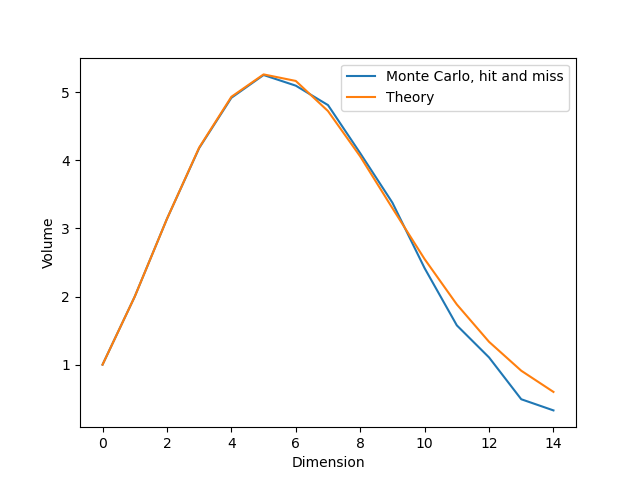
\includegraphics[width=1\textwidth]{q1.png}
    \caption{More hyperspheres, volume to dimension. When $d$ larger than $10$, the error is noticable.}
    \label{fig:q1}
\end{figure}

\subsection{Pseudocode}
\begin{algorithm}[H]% the algorithm block floats in the page 
\caption{Volume of hypersphere}
    \begin{algorithmic}[1]% This number indicates the line number to start labeling with line number.
        \Statex\textbf{Input:} dimension $d$
        \Statex\textbf{Output:} volume of the hypersphere calculated by the Monte-Carlo method.
        \State $N \gets 1\times 10^{4}$
        \State $n\gets 0$
        \For{$i$ in range(N)}
        		\State generate a random $d$-dimensional vector $\vec{x}$, each component distributed linearly in $[-1/2, 1/2)$
        		\If{$\|\vec{x}\| < 1$}
        			\State $n \gets n + 1$
        		\EndIf
        \EndFor
	\Statex\textbf{Return:} $n / N$
    \end{algorithmic}
\end{algorithm}

\section{3D Classical Heisenburg Model }
\subsection{Problem Description}
Write a MC code for a 3D Face-Centered Cubic lattice using the Heisenberg spin model (adopt periodic boundary condition). Estimate the ferromagnetic Curie temperature. The Hamiltonian is $H=-J\sum__{\langle i,j\rangle}\vec{s}_i\cdot \vec{s}_j$ where $J=1$.

\subsection{Solution}
We adopted the typical scheme for MC simulation:
\begin{itemize}
	\item Choose a spin at random
	\item Change the selected spin at random
	\item Calculate the energy change introduced by the above change
	\item Accept the change at a probability of $e^{-\Delta E\over k_B T}$
	\item loop the above steps until equilibrium is reached.
\end{itemize}
In fact, the acceptance rate corresponds to the 

\end{document}